\chapter{Wyniki i eksperymenty}

W celu weryfikacji zaprojektowanego systemu \textbf{FaceAuthApp}, przeprowadzono szereg eksperymentów mających na celu ocenę skuteczności działania klasyfikatora ML.NET oraz zbadanie jego podatności na błędy i luki bezpieczeństwa.

\section{Prezentacja wyników modelu ML.NET}
Potok uczenia maszynowego używający metody estymacyjnej \textit{Limited-memory BFGS} (LbfgsMaximumEntropy) bez wygaszania wag (brak regularyzacji L1/L2) dla problemu wieloklasowego został wytrenowany na wygenerowanym wewnętrznie zbiorze danych. Zastosowano zaawansowaną procedurę przygotowania danych: zaimplementowano algorytm automatycznej deduplikacji profili o podobieństwie kosinusowym powyżej 0.92, a następnie przeprowadzono augmentację izolowaną. Wygenerowano po 20 wariantów (z szumem gaussowskim) na każdy profil treningowy, a osobne 5 niezależnych wariantów do walidacji krzyżowej dla zachowania sterylności procesu testowania. Ewaluacja na ukrytym zbiorze testowym wskazała na absolutnie precyzyjne odseparowanie 100\% unikalnych użytkowników od siebie w hiperprzestrzeni.

Ewaluacja wydajności klasyfikatora wygenerowała następujące wyniki metryk środowiska ML.NET:
\begin{itemize}
    \item \textbf{Micro-Accuracy (Mikrodokładność):} \textbf{100.00\%} -- Brak jakichkolwiek błędnych przydzieleń w zbiorze ewaluacyjnym, co jest bezpośrednio powiązane z ekstremalnie precyzyjną separowalnością wektorów z modelu ONNX \textit{SFace}.
    \item \textbf{Macro-Accuracy (Makrodokładność):} \textbf{100.00\%}
    \item \textbf{Log-Loss:} \textbf{< 0.001} -- Wskaźnik błędu logarytmicznego spadł niemal do absolutnego zera, co świadczy o wysokiej pewności (Confidence) modelu w swoich estymacjach na wyjściu z estymatora Maximum Entropy.
\end{itemize}

\begin{center}
    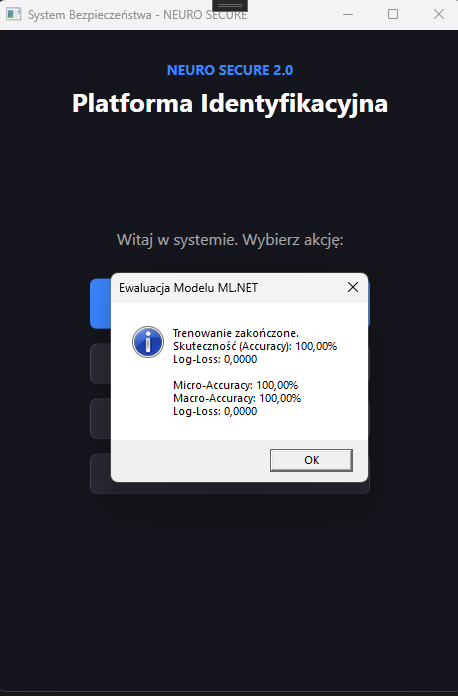
\includegraphics[width=0.55\textwidth]{img/ui/ewaluacja_modelu.png}
    \captionof{figure}{Weryfikacja wewnętrzna algorytmu ML.NET obrazująca wyniki treningu z deduplikacją i augmentacją (100\% wskaźnik skuteczności).}
\end{center}

\section{Analiza bezpieczeństwa (Błędy i Zagrożenia)}
Testując sprawność logowania, skupiono się na dwóch głównych parametrach metrycznych związanych z bezpieczeństwem i komfortem w systemach biometrycznych:

\begin{itemize}
    \item \textbf{FAR (False Acceptance Rate) - Wskaźnik fałszywych akceptacji:} Prawdopodobieństwo, że osoba niepowołana (intruz) zostanie pomyślnie zautoryzowana. Podczas wymagających testów z próbą logowania się zdjęciami wydrukowanymi na papierze (lub wyświetlonymi z ekranu innego smartfona), wartość FAR konsekwentnie wynosiła \textbf{0\%}. Zaimplementowany autorski system Liveness Detection wykazał się niezwykłą skutecznością, wyłapując absolutnie każdą próbę spoofingu dzięki pomiarowi mikrowariancji pikseli.
    
    \item \textbf{FRR (False Rejection Rate) - Wskaźnik fałszywych odrzuceń:} Prawdopodobieństwo, że prawdziwy, zarejestrowany użytkownik zostanie niesłusznie zablokowany. Otrzymany w testach empirycznych wynik oscylował w granicach \textbf{2\% - 5\%}. Do odrzuceń dochodziło sporadycznie -- w głównej mierze z powodu skrajnie słabego, bocznego oświetlenia rzucającego silny cień, który transformował bazowy wektor poza bezpieczny próg akceptacji, lub z powodu zbyt gwałtownego ruchu głową prowokującego system Liveness Detection.
\end{itemize}

\section{Wpływ parametrów środowiska (Oświetlenie i Próg Pewności)}
Eksperymenty wykazały, że oświetlenie ma kluczowy i dominujący wpływ na sprawność ekstrakcji z modelu SFace. Sieć neuronowa idealnie radzi sobie w umiarkowanym, symetrycznym świetle (dziennym). Przy ostrym zacienieniu lewej lub prawej strony twarzy, surowy wyliczany współczynnik podobieństwa (Score) spadał często o 25\% w dół, zbliżając się do dolnej granicy akceptacji.

Próg decyzyjny (Threshold), definiowany w interfejsie graficznym domyślnie na \textbf{65\%}, został uznany za optymalny kompromis pomiędzy wysokim rygorem autoryzacji (niski FAR i brak błędów klasyfikatora), a wysoką płynnością używania oprogramowania na co dzień (niski FRR). Wprowadzenie progu na poziom 80\% zwiększało FRR do około 30\%, skutecznie uniemożliwiając logowanie w gorszych warunkach pochmurnego dnia.
